\setcounter{equation}{0}
\chapter{Proposed Methodology}
\label{chap:methodology}

The methodology combines a data-rescue procedure for the register with a staged transfer-learning procedure for the forecast. The two tracks share one repository\footnote{\url{https://github.com/CSVaishakh/TransferLearningBasedWeatherForecasting}} and communicate only through files on disk: digitization writes \textbf{sjcet\_daily.csv}, the model reads it and writes its forecasts and metrics, and a web application serves those files. Each track can therefore be rerun or replaced without touching the others.

\section{System Workflow}
\label{sec:workflow}

The work follows the plan presented at the zeroth review, \textsc{Digitize $\to$\allowbreak{} Analyse $\to$\allowbreak{} Predict $\to$\allowbreak{} Integrate $\to$\allowbreak{} Validate} (Figure~\ref{fig:pipeline}). The register pages are transcribed and validated into a single quality-flagged daily file; regional reanalysis, reference stations and the register are joined into one graph; the forecasting network is trained in three stages alongside the baselines; and replay and live forecasts are served through a FastAPI backend and a React web application, where each forecast can be compared with what the register recorded.

\begin{figure}[!htbp]
    \centering
    \begin{tikzpicture}[
        every node/.style={font=\scriptsize},
        wkstep/.style={draw=brandbrown, rounded corners=3pt, minimum width=2.7cm,
                       minimum height=1.0cm, fill=brandbeige, align=center,
                       text width=2.5cm, inner sep=3pt},
        file/.style={draw=brandrule, fill=brandcream, rounded corners=1pt, align=center,
                     font=\tiny\ttfamily, inner sep=2pt, text width=2.5cm},
        arrow/.style={-{Latex[length=2.4mm]}, brandbrown, line width=0.8pt},
        phase/.style={font=\scriptsize\bfseries, text=brandtan, align=center}
    ]
        \node[wkstep] (s1) at (0,0) {1. Digitize\\register pages};
        \node[wkstep, right=0.5cm of s1] (s2) {2. Validate \&\\assemble};
        \node[wkstep, right=0.5cm of s2] (s3) {3. Analyse\\the record};
        \node[wkstep, right=0.5cm of s3] (s4) {4. Build regional\\dataset \& graph};

        \node[wkstep] (s5) at (1.6,-2.7) {5. Staged\\training};
        \node[wkstep, right=0.5cm of s5] (s6) {6. Replay \& live\\forecasts};
        \node[wkstep, right=0.5cm of s6] (s7) {7. Present \&\\validate (web app)};

        \draw[arrow] (s1) -- (s2);
        \draw[arrow] (s2) -- (s3);
        \draw[arrow] (s3) -- (s4);
        \draw[arrow] (s4.south) -- ++(0,-0.6) -| (s5.north);
        \draw[arrow] (s5) -- (s6);
        \draw[arrow] (s6) -- (s7);

        \node[file, below=0.15cm of s1] {transcripts/mNN.csv};
        \node[file, below=0.15cm of s2] {sjcet\_daily.csv};
        \node[file, below=0.15cm of s5] {runs/*/best.pt};
        \node[file, below=0.15cm of s6] {forecasts/*.json};
        \node[file, below=0.15cm of s7] {localhost:5173};

        \draw[decorate, decoration={brace, amplitude=4pt}, brandtan, line width=0.6pt]
            ($(s1.north west)+(-0.05,0.18)$) -- ($(s3.north east)+(0.05,0.18)$);
        \node[phase, above=0.28cm] at ($(s1.north)!0.5!(s3.north)$) {Digitization track};
        \draw[decorate, decoration={brace, amplitude=4pt}, brandtan, line width=0.6pt]
            ($(s4.north west)+(-0.05,0.18)$) -- ($(s4.north east)+(0.05,0.18)$);
        \node[phase, above=0.28cm] at (s4.north) {Model track};
    \end{tikzpicture}
    \caption{\capFigPipeline}\label{fig:pipeline}
\end{figure}

\section{Data Sources}
\label{sec:sources}

\footnotesize
\begin{longtable}{|L{2.33cm}|L{5.02cm}|L{4.48cm}|}
\caption{\capTabSources}\label{tab:sources}\\
\hline
\textbf{Source} & \textbf{Content} & \textbf{Used for} \\
\hline
\endfirsthead
\hline
\textbf{Source} & \textbf{Content} & \textbf{Used for} \\
\hline
\endhead
SJCET weather register & Daily dry/wet bulb, max/min temperature and rainfall, Jul 2010 -- Dec 2016 (digitized by this work) & Stage-3 target; History page \\ \hline
NASA POWER & Daily MERRA-2-based reanalysis \cite{ref15}, 1990--2025: 1\textdegree{} over India, 0.5\textdegree{} over Kerala, plus a point at SJCET & Stage-1 pretraining; live inputs \\ \hline
NOAA GSOD \cite{ref12} & Daily station summaries: Bangalore, Coimbatore, Mangalore, Thiruvananthapuram, Kozhikode, Cochin & Stage-2 pretraining; live inputs \\ \hline
ERA5 (planned) & Hourly reanalysis aggregated to daily statistics & Not used: the Copernicus queue was too slow; downloader kept \\ \hline
\end{longtable}
\normalsize

\textbf{NASA POWER reanalysis.} The original plan used ERA5 daily statistics, but Copernicus requests sat in the queue for over an hour without starting. NASA POWER returns 36 years of daily data for one point in about four seconds without an API key, and was adopted instead; its resolution of about 0.5\textdegree{} set the resolution of the Kerala grid. Nine variables are taken for every grid node: daily maximum, minimum and mean 2-m temperature, 2-m dewpoint, precipitation, surface pressure, the $u$ and $v$ components of 10-m wind, and cloud amount. The India box spans 6--37\textdegree N, 68--98\textdegree E at 1\textdegree; the Kerala box spans 8--13\textdegree N, 74--78\textdegree E at 0.5\textdegree.

\textbf{NOAA GSOD stations.} Units are converted from \textdegree F and inches, incomplete precipitation totals are dropped, and basic range checks are applied (maximum 15--45\,\textdegree C, minimum 5--35\,\textdegree C, rain at most 500\,mm). Stations with less than 50\% coverage are excluded, leaving six.

\section{Digitization of the SJCET Register}
\label{sec:digitization}

The clean source is a scanned PDF with one page per month from July 2010 to December 2016 (78 months). A separate summary PDF gives the rainfall of each month and year, and a further 289 phone photographs cover later years and are not yet transcribed. Following the practice of historical data rescue \cite{ref1,ref2,ref3}, each page was processed as follows:

\begin{enumerate}
    \item \textbf{Transcribe} every cell exactly as written into one CSV per page, with a header giving the year, month and column order (two layouts occur, one up to 2011 and one from 2012).
    \item \textbf{Check} each page automatically: the row count matches the days in the month, values fall in physical ranges, the wet bulb does not exceed the dry bulb, the minimum is below the maximum, and the rain column sums to the written total.
    \item \textbf{Re-read} disagreements zoomed in, and decide whether the error is ours or the observer's.
    \item \textbf{Assemble} all pages onto a complete calendar, converting rain to millimetres, deriving relative humidity, and storing a flag and note for every row.
\end{enumerate}

A row is flagged \textbf{suspect} if its remarks describe a value as doubtful, unreadable or overwritten, if it breaks physics as written, if its rain may be accumulated over unobserved days, or if its month disagrees with the written total. The flag never deletes a value; it records the reason so that the modelling step can decide what to drop. Blank rain cells are stored as \textbf{not recorded}, never as zero.

\textbf{Rainfall checksums.} Together, the foot of the rain column (2014--2016) and the summary pages give a written total for every month. \textbf{59 of 78 months} match it to within 0.1\,cm. For six mismatched months a zoomed re-read confirmed the digits as transcribed, so these are addition errors by the observer; in the remaining months every rain value is kept but flagged.

\label{sec:dig-oddities}\textbf{Oddities.} The register has its own quirks: min/max headers swapped from 20 June 2011, dates written as ``-10'' in September 2011, ink bleed-through in June 2013, blank daily pages for November and December 2012 although the summary gives totals for both, and a maximum temperature that is often constant for weeks (for example 34\,\textdegree C every day of January 2013), which suggests the maximum thermometer was reset irregularly. The register yields 1,549 observed days in 2,376 calendar days (65\%), with weekends and holidays accounting for most gaps (Figure~\ref{fig:coverage}).

\begin{figure}[!htbp]
    \centering
    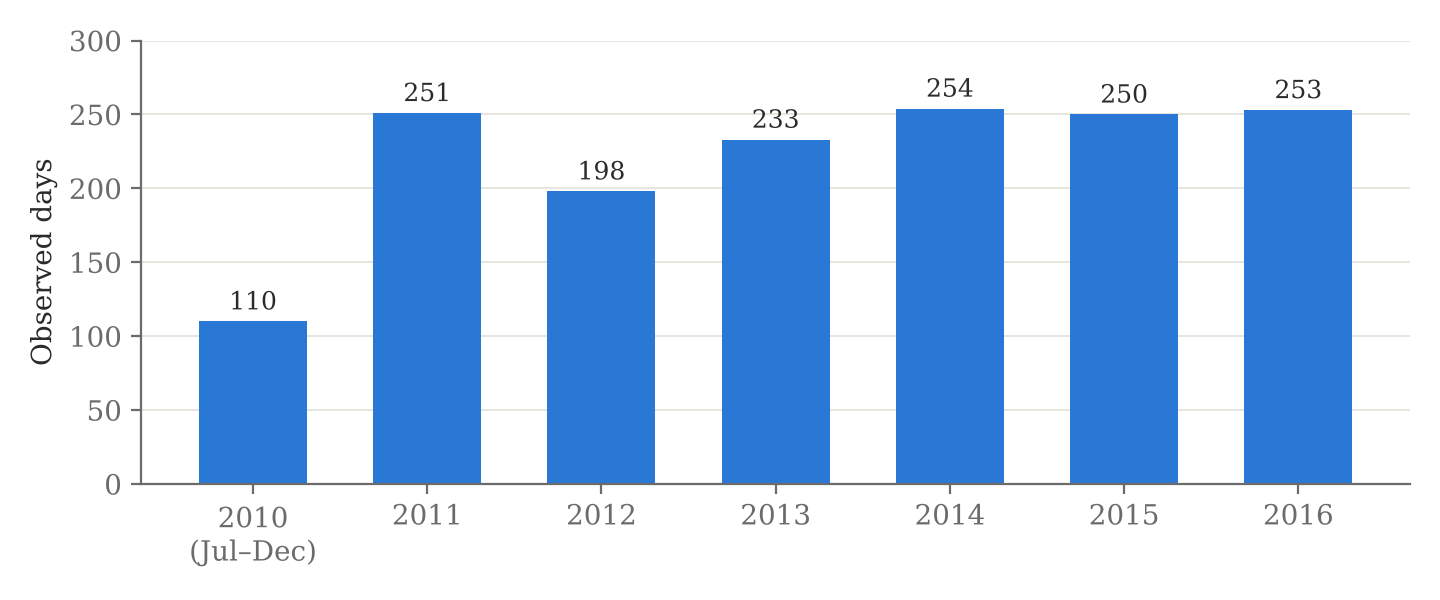
\includegraphics[width=0.85\textwidth]{register_coverage.png}
    \caption{\capFigCoverage}\label{fig:coverage}
\end{figure}

\label{sec:ocr}\textbf{Why not OCR.} The proposal planned an OCR route with table structure recognition \cite{ref2,ref4} and a handwriting recogniser. On 150 hand-labelled cells, zero-shot TrOCR \cite{ref11} read at best 35.3\% exactly (character error rate 0.48), and fine-tuning it needs a GPU the team did not have. For 78 months of pages, manual transcription with automatic checks was faster and more reliable, and, since table-recognition models depend on large labelled training sets \cite{ref10}, the transcripts now form a complete labelled set for training an OCR model \cite{ref3} on the later photographs.

\section{Preparing the Register for Modelling}
\label{sec:sjcet-handling}

The register is added to the graph as one station node, with four adjustments:

\begin{itemize}
    \item \textbf{08:30 reading convention.} Rain recorded on date $D$ fell between 08:30 on $D-1$ and 08:30 on $D$, and the maximum thermometer read on $D$ holds the maximum of $D-1$; both are moved to $D-1$, while the minimum stays on $D$.
    \item \textbf{Dewpoint} is computed from the 08:30 dry/wet-bulb pair (Equations~(\ref{eq:es})--(\ref{eq:td})); the daily mean is approximated as $(T_{\max}+T_{\min})/2$.
    \item \textbf{Suspect values} lose their rain value, and also their temperatures when the doubt concerns a reading rather than a monthly rain mismatch.
    \item \textbf{Accumulated rain.} A reading after an unread day contains several days of rain, so it is dropped rather than attributed to a single day.
\end{itemize}

With the dry-bulb temperature $T$ and the wet-bulb temperature $T_w$ in \textdegree C and a station pressure of about 1005\,hPa, the saturation vapour pressure, the actual vapour pressure and the dewpoint are
\begin{equation}
e_s(x)=6.112\,\exp\!\left(\frac{17.67\,x}{x+243.5}\right),
\label{eq:es}
\end{equation}
\begin{equation}
e=e_s(T_w)-0.000799\times1005\,(T-T_w),
\label{eq:e}
\end{equation}
\begin{equation}
T_d=\frac{243.5\,\ln(e/6.112)}{17.67-\ln(e/6.112)}.
\label{eq:td}
\end{equation}

After these steps the training period contains 716 SJCET temperature days and 249 rain days (July 2010 -- 2013); 2014 is used for validation and 2015--2016 for testing.

\section{Forecasting Model}
\label{sec:model}

\textbf{The weather graph.} Every source is assembled onto one daily calendar from 1990 to 2025 and every node is connected to its eight nearest neighbours by great-circle distance (Table~\ref{tab:graph}). Each edge carries the east--west and north--south offsets, the distance and the elevation difference. A graph \cite{ref7,ref13} accepts the coarse India grid, the fine Kerala grid, the irregular stations and SJCET as they are, without interpolation, and makes the transfer natural: SJCET is simply another node, hidden in stages 1 and 2 and revealed in stage 3.

\begin{table}[!htbp]
    \centering
    \caption{\capTabGraph}\label{tab:graph}
    \footnotesize
    \begin{tabularx}{\textwidth}{|L{4.4cm}|C{1.6cm}|Y|}
        \hline
        \textbf{Node group} & \textbf{Count} & \textbf{Notes} \\ \hline
        Reanalysis, India 1\textdegree & 962 & Coarse context; loss weight 0.1 in stage 2 \\ \hline
        Reanalysis, Kerala 0.5\textdegree & 99 & Fine grid around the target \\ \hline
        Reanalysis point at SJCET & 1 & Reanalysis value at the campus location \\ \hline
        NOAA GSOD stations & 6 & Real observations; loss weight 2 in stage 2 \\ \hline
        SJCET register & 1 & Hidden in stages 1--2; the only loss node in stage 3 \\ \hline
        \textbf{Total} & \textbf{1,069} & $k=8$ nearest neighbours, symmetrised \\ \hline
    \end{tabularx}
\end{table}

\textbf{Inputs and outputs.} Table~\ref{tab:io} lists what each node sees and predicts. Each variable is normalised with statistics from the stage-1 training years on reanalysis nodes,
\begin{equation}
\tilde{x}_{v,t,k}=\frac{g_k(x_{v,t,k})-\mu_k}{\sigma_k}, \qquad g_k(x)=\begin{cases}\log(1+x) & k=\text{rain}\\ x & \text{otherwise}\end{cases}
\label{eq:norm}
\end{equation}
and missing values are set to zero and flagged by a separate mask channel, so the model learns the difference between ``zero'' and ``unknown''. This matters because SJCET is missing on every weekend and holiday. Relative humidity is derived from the forecast mean temperature $T$ and dewpoint $T_d$,
\begin{equation}
\mathrm{RH}=100\,\frac{E(T_d)}{E(T)}, \qquad E(x)=6.112\,\exp\!\left(\frac{17.62\,x}{243.12+x}\right).
\label{eq:rh}
\end{equation}

\begin{table}[!htbp]
    \centering
    \caption{\capTabIO}\label{tab:io}
    \footnotesize
    \begin{tabularx}{\textwidth}{|L{2.6cm}|Y|}
        \hline
        \textbf{Inputs} & Last 7 days of 9 variables (tmax, tmin, tmean, dewpoint, rain, surface pressure, $u_{10}$, $v_{10}$, cloud), normalised; the matching 7$\times$9 missing-value mask; latitude, longitude, elevation, node type (reanalysis/station); and the day of year of the first forecast day as $(\sin,\cos)$. \\ \hline
        \textbf{Outputs} & For each lead day $d=1,\dots,6$: tmax, tmin, rain ($\log(1+x)$), tmean, dewpoint, and a logit for rain $\geq$ 2.5\,mm (the IMD rainy-day threshold). \\ \hline
        \textbf{Derived} & Relative humidity, from the forecast tmean and dewpoint with the Magnus formula; it is not predicted directly. \\ \hline
    \end{tabularx}
\end{table}

\textbf{Network.} \textbf{WeatherGNN} follows the encode--process--decode pattern of graph-based weather models (Figure~\ref{fig:gnn}). A two-layer MLP encodes each node into a 128-dimensional state; four processor blocks each apply layer normalisation, a GATv2 convolution \cite{ref13} with four heads and edge features, and a feed-forward block, both with residual connections; and an MLP decoder emits all six lead days at once, which avoids error accumulation. The model has about 0.4\,M parameters and trains on a CPU. Each processor block updates the hidden state $h_i$ of node $i$ as
\begin{align}
h_i &\leftarrow h_i + \mathrm{Drop}\big(\mathrm{GATv2}(\mathrm{LN}(h))_i\big), \label{eq:block1}\\
h_i &\leftarrow h_i + \mathrm{Drop}\big(\mathrm{FFN}(h_i)\big), \label{eq:block2}
\end{align}
where the GATv2 layer \cite{ref13} aggregates the neighbours $j\in\mathcal{N}(i)$ with attention weights computed from both node states and the edge features $e_{ij}$:
\begin{equation}
\alpha_{ij}=\operatorname*{softmax}_{j\in\mathcal{N}(i)}\Big(a^{\top}\,\mathrm{LeakyReLU}\big(\Theta_s h_i+\Theta_t h_j+\Theta_e e_{ij}\big)\Big), \qquad
\mathrm{GATv2}(h)_i=\sum_{j\in\mathcal{N}(i)}\alpha_{ij}\,\Theta_t h_j .
\label{eq:gat}
\end{equation}

\begin{figure}[!htbp]
    \centering
    \begin{tikzpicture}[
        every node/.style={font=\scriptsize},
        blk/.style={draw=brandbrown, rounded corners=2pt, fill=brandbeige, align=center, minimum height=0.9cm, text width=2.1cm},
        io/.style={draw=brandrule, rounded corners=2pt, fill=brandcream, align=center, minimum height=0.9cm, text width=2.0cm},
        arrow/.style={-{Latex[length=2mm]}, brandbrown, line width=0.8pt}
    ]
        \node[io] (x) at (0,0) {Node features\\(7 d $\times$ 9 vars\\+ mask + static)};
        \node[blk, right=0.45cm of x] (enc) {Encoder\\MLP $\to$\allowbreak{} 128};
        \node[blk, right=0.45cm of enc, text width=3.0cm, minimum height=1.6cm] (proc) {\textbf{$\times$4 processor}\\LayerNorm $\to$\allowbreak{} GATv2\\(4 heads, edge feats) + res.\\LayerNorm $\to$\allowbreak{} FFN + res.};
        \node[blk, right=0.45cm of proc] (dec) {Decoder\\MLP $\to$\allowbreak{} 6$\times$6};
        \node[io, right=0.45cm of dec] (y) {tmax, tmin, rain,\\tmean, td, P(rain)\\for d = 1..6};
        \draw[arrow] (x) -- (enc); \draw[arrow] (enc) -- (proc); \draw[arrow] (proc) -- (dec); \draw[arrow] (dec) -- (y);
        \node[io, below=0.5cm of proc, text width=3.0cm, minimum height=0.6cm] (g) {Graph: 1,069 nodes, $k$=8};
        \draw[arrow] (g) -- (proc);
    \end{tikzpicture}
    \caption{\capFigGnn}\label{fig:gnn}
\end{figure}

\textbf{Loss.} The loss is a masked, node-weighted mean squared error over the regression targets plus half a weighted binary cross-entropy for rain occurrence,
\begin{equation}
\mathcal{L} = \frac{\sum m\,w\,(\hat{y}-y)^2}{\sum m\,w} \;+\; 0.5\,\frac{\sum m\,w\,\mathrm{BCE}_{p^{+}=2}(\hat{z},o)}{\sum m\,w},
\label{eq:loss}
\end{equation}
where $m$ is the target mask, $w$ the per-node stage weight, $\hat{z}$ the rain logit and $o$ the observed occurrence. A missing target contributes nothing.

\section{Staged Transfer Learning}
\label{sec:stages}

Each stage of the transfer \cite{ref7,ref8} closes a different gap (Figure~\ref{fig:method}, Table~\ref{tab:stages}). Stage 1 learns \textbf{weather}: how the nine variables evolve over seven days across India. Stage 2 learns the \textbf{observation gap}: how real thermometers and rain gauges differ from reanalysis in the region. Stage 3 learns \textbf{SJCET}: its 08:30 convention, its whole-degree readings and its slope location. The splits are identical in every stage, and the checkpoint with the lowest validation loss is kept.

\begin{figure}[!htbp]
    \centering
    \begin{tikzpicture}[
        every node/.style={font=\scriptsize},
        box/.style={draw=brandbrown, rounded corners=3pt, fill=brandbeige, align=center,
                    text width=3.5cm, minimum height=2.3cm, inner sep=4pt},
        src/.style={draw=brandrule, rounded corners=2pt, fill=brandcream, align=center,
                    text width=3.5cm, inner sep=3pt},
        arrow/.style={-{Latex[length=2.4mm]}, brandbrown, line width=0.9pt},
    ]
        \node[box] (b1) at (0,0) {\textbf{Stage 1: Region}\\[1mm] 1,062 reanalysis nodes\\ India 1\textdegree, Kerala 0.5\textdegree\\[1mm] loss on all reanalysis nodes\\ 4 epochs, lr $10^{-3}$};
        \node[box, right=0.9cm of b1] (b2) {\textbf{Stage 2: Stations}\\[1mm] + 6 NOAA GSOD stations\\[1mm] loss: Kerala grid ($\times$1), stations ($\times$2), India grid ($\times$0.1)\\ 4 epochs, lr $3{\times}10^{-4}$};
        \node[box, right=0.9cm of b2] (b3) {\textbf{Stage 3: SJCET}\\[1mm] + SJCET node, fraction $\phi$ of its training months\\[1mm] loss on SJCET only, 4-hop subgraph\\ 25 epochs, lr $10^{-4}$};
        \draw[arrow] (b1) -- node[above]{weights} (b2);
        \draw[arrow] (b2) -- node[above]{weights} (b3);
        \node[src, below=0.45cm of b1] {NASA POWER 1990--2025\\(MERRA-2 based)};
        \node[src, below=0.45cm of b2] {NOAA GSOD 1990--2025};
        \node[src, below=0.45cm of b3] {Digitized register\\Jul 2010 -- Dec 2016};
        \node[draw=brandtan, dashed, rounded corners=3pt, fill=white, text width=12.5cm, align=center, inner sep=4pt]
            at (4.4,-3.2) {\textbf{Ablation:} three strategies (scratch, 1$\to$\allowbreak{}3, 1$\to$\allowbreak{}2$\to$\allowbreak{}3) $\times$ $\phi\in\{10,25,50,100\%\}$ $\times$ 3 seeds; baselines on the same test days.\\
            \textbf{Splits:} train 1990--2013 \quad validation 2014 \quad test 2015--2016 (identical in every stage).};
    \end{tikzpicture}
    \caption{\capFigMethod}\label{fig:method}
\end{figure}

\begin{table}[!htbp]
    \centering
    \caption{\capTabStages}\label{tab:stages}
    \footnotesize
    \begin{tabularx}{\textwidth}{|C{1.1cm}|L{4.2cm}|Y|}
        \hline
        \textbf{Stage} & \textbf{Data the model sees} & \textbf{Loss on} \\ \hline
        1 & Reanalysis nodes only & All reanalysis nodes (weight 1) \\ \hline
        2 & + NOAA stations (SJCET still hidden) & Kerala 0.5\textdegree{} nodes (1), stations (2), India 1\textdegree{} nodes (0.1) \\ \hline
        3 & + SJCET, a fraction $\phi$ of its training months & SJCET only, on its 4-hop subgraph \\ \hline
    \end{tabularx}
\end{table}

Because the network has four message-passing layers, only nodes within four hops of SJCET can influence its output, so stage 3 runs on that subgraph alone. The fraction $\phi$ is applied to whole months, shuffled with the run's seed, so a 10\% run sees a few complete months rather than scattered days. Table~\ref{tab:hyper} gives the training settings.

\begin{table}[!htbp]
    \centering
    \caption{\capTabHyper}\label{tab:hyper}
    \footnotesize
    \begin{tabularx}{\textwidth}{|L{4.6cm}|Y|}
        \hline
        \textbf{Setting} & \textbf{Value} \\ \hline
        Input window / horizon & 7 days / 6 lead days \\ \hline
        Hidden size, layers, heads, dropout & 128, 4, 4, 0.1 \\ \hline
        Optimiser & AdamW, weight decay $10^{-4}$, gradient clipping at 1.0 \\ \hline
        Schedule & One-cycle learning rate, 10\% warm-up \\ \hline
        Epochs / learning rate & Stage 1: 4 / $10^{-3}$ (continued from a one-day-horizon model); stage 2: 4 / $3{\times}10^{-4}$; stage 3: 25 / $10^{-4}$ (pretrained) or $10^{-3}$ (scratch) \\ \hline
        Batch / steps per epoch & 16 random days / up to 150 batches \\ \hline
        Early stopping & Patience 4 epochs on validation loss; best checkpoint kept \\ \hline
        Seeds & 0, 1, 2 for fractions below 100\%; seed 0 at 100\% \\ \hline
    \end{tabularx}
\end{table}

\label{sec:method-missing}\textbf{Missing data.} A seven-day input window at SJCET usually has two or more missing days. Inputs are handled by the mask channel and targets by masking the loss. An optional variant (\textbf{-{}-clim-fill}) feeds a smoothed day-of-year climatology of SJCET in place of missing inputs while keeping the mask set to ``missing''.

\label{sec:live}\textbf{Live forecasting.} \textbf{live.py} fetches recent NASA POWER data for SJCET's 4-hop neighbourhood and the latest GSOD files, builds the seven-day window ending on the last complete day, and runs the default region$\to$\allowbreak{}stations$\to$\allowbreak{}SJCET model. NASA POWER publishes about three days late, so today is usually lead day 4, which is why the horizon was extended to six days. Because the register stops in 2016, SJCET's own inputs are empty in a live forecast; a live-like test (Section~\ref{sec:res-livelike}) measures the effect.

\section{Evaluation Setup}
\label{sec:evaluation}

Four baselines, including XGBoost \cite{ref14}, are scored on exactly the same SJCET test days and, where they use training data, the same subset of training months as the GNN they are compared with (Table~\ref{tab:baselines}).

\begin{table}[!htbp]
    \centering
    \caption{\capTabBaselines}\label{tab:baselines}
    \footnotesize
    \begin{tabularx}{\textwidth}{|L{2.6cm}|Y|}
        \hline
        \textbf{Baseline} & \textbf{Definition} \\ \hline
        Persistence & Every lead day equals today's SJCET observation (``tomorrow = today''). Scored only on days that follow a reading. \\ \hline
        Climatology & Day-of-year mean of SJCET's training months, smoothed over $\pm$15 days. \\ \hline
        Reanalysis & NASA POWER value at the nearest grid node on the target day. It is not a forecast; it shows how far gridded reanalysis is from the station even with perfect knowledge of the day. \\ \hline
        XGBoost \cite{ref14} & SJCET's last 7 days of five variables plus the nearest grid node's last 7 days of nine variables plus the day of year; one model per lead day and target (300 trees, depth 5, learning rate 0.05). \\ \hline
        GNN from scratch & The same network and stage-3 procedure with random initial weights, serving as the control for pretraining. \\ \hline
    \end{tabularx}
\end{table}

For $n$ test days with forecasts $\hat{y}_i$ and observations $y_i$ the main scores are
\begin{equation}
\mathrm{RMSE}=\sqrt{\frac{1}{n}\sum_{i=1}^{n}(\hat{y}_i-y_i)^2}, \qquad \mathrm{MAE}=\frac{1}{n}\sum_{i=1}^{n}\lvert\hat{y}_i-y_i\rvert,
\label{eq:rmse}
\end{equation}
\begin{equation}
\mathrm{Bias}=\frac{1}{n}\sum_{i=1}^{n}(\hat{y}_i-y_i), \qquad R^2=1-\frac{\sum_i(\hat{y}_i-y_i)^2}{\sum_i(y_i-\bar{y})^2},
\label{eq:bias}
\end{equation}
and, for the rain probability $p_i$ and observed occurrence $o_i\in\{0,1\}$, the Brier score is $\frac{1}{n}\sum_i(p_i-o_i)^2$. Forecast \textbf{accuracy}, the primary result, is reported as $100-\mathrm{MAPE}$ for temperature together with the share of forecasts within $\pm$1 and $\pm$2\,\textdegree C of the register reading; rain occurrence ($\geq$2.5\,mm) is scored by rain/no-rain accuracy, hit rate and false-alarm ratio. All metrics are computed in physical units at the SJCET node, separately for each lead day. Four experiments are run: a \textbf{full-data comparison} with all SJCET training months; a \textbf{data-efficiency ablation} over three strategies, four fractions and three seeds; a \textbf{live-like test} with SJCET's own inputs hidden; and a \textbf{seasonal breakdown} of the day-1 error.
